\renewcommand{\thesection}{\Alph{section}}

\begin{appendices}
\chapter{Information References}

\section{\ac{epc} Schemes and Corresponding GS1 keys} \label{anx:epccodingschemes}
\begin{table}[!ht]
    \centering
    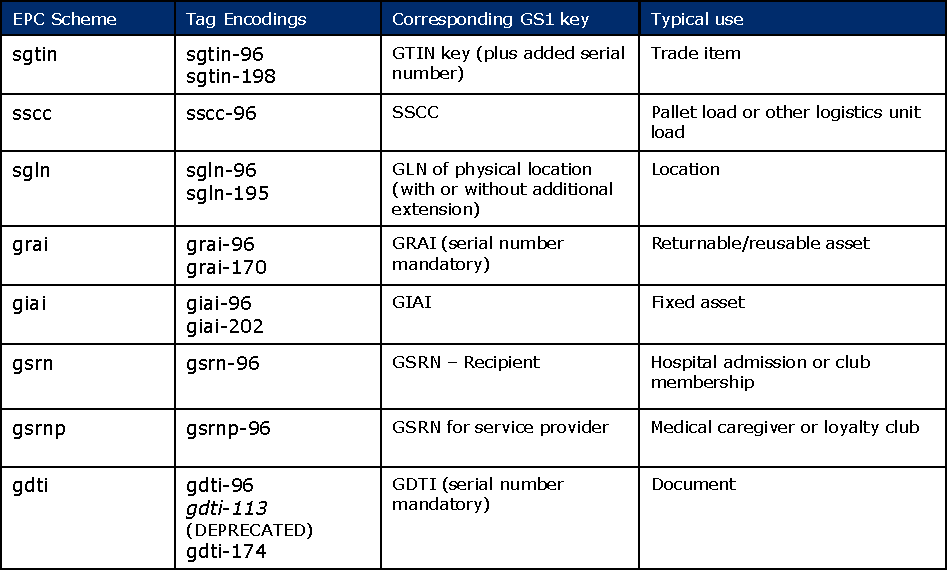
\includegraphics[width=\textwidth]{./figs/02-state-of-the-art/epcschemes.pdf}
    \caption{\ac{epc} Schemes and Corresponding GS1 keys}
\end{table}

\begin{table}
    \centering
    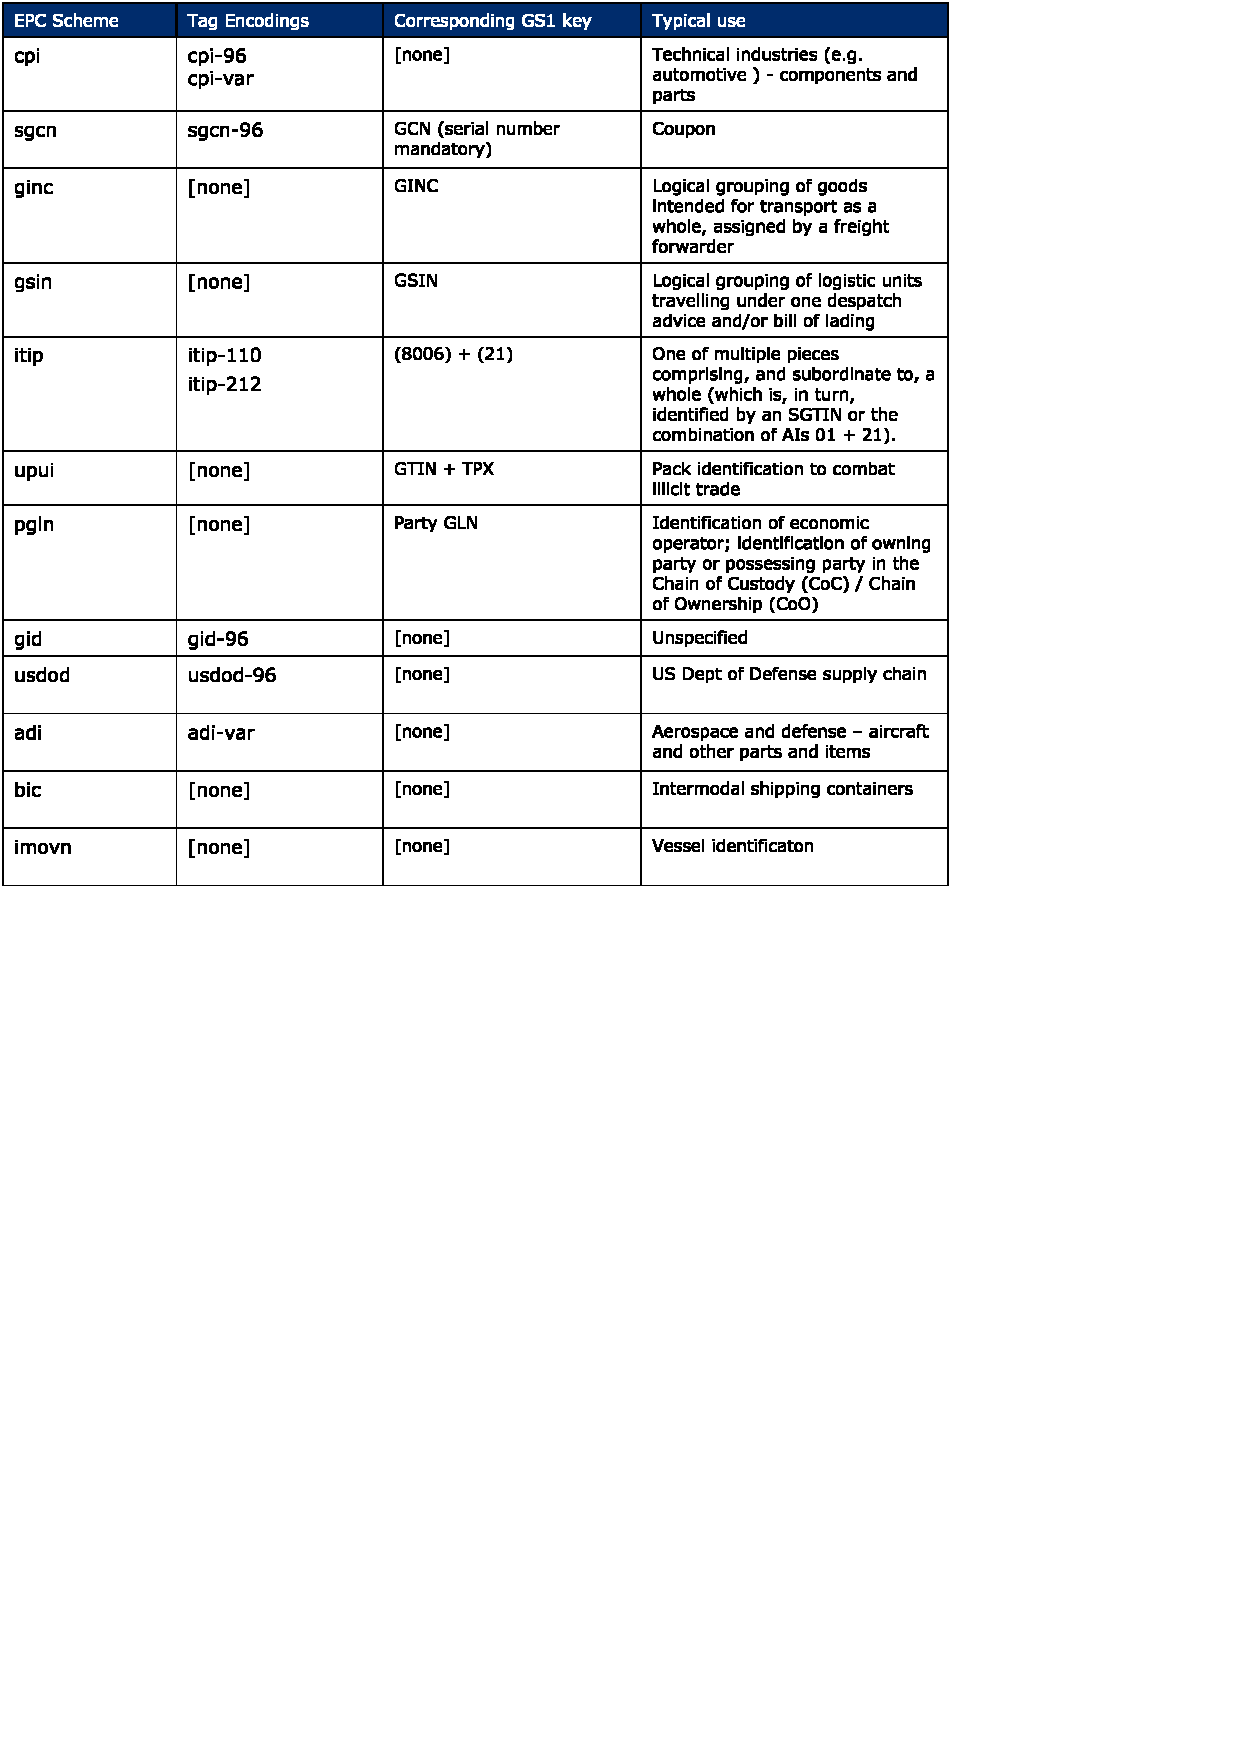
\includegraphics[width=\textwidth]{./figs/02-state-of-the-art/epcschemes2.pdf}
    \caption{\ac{epc} Schemes and Corresponding GS1 keys~\cite{EPCTagData}}
\end{table}

\clearpage

\section{\ac{llrp} Messages} \label{anx:llrpmessages}
\begin{table}[!ht]
    \centering
    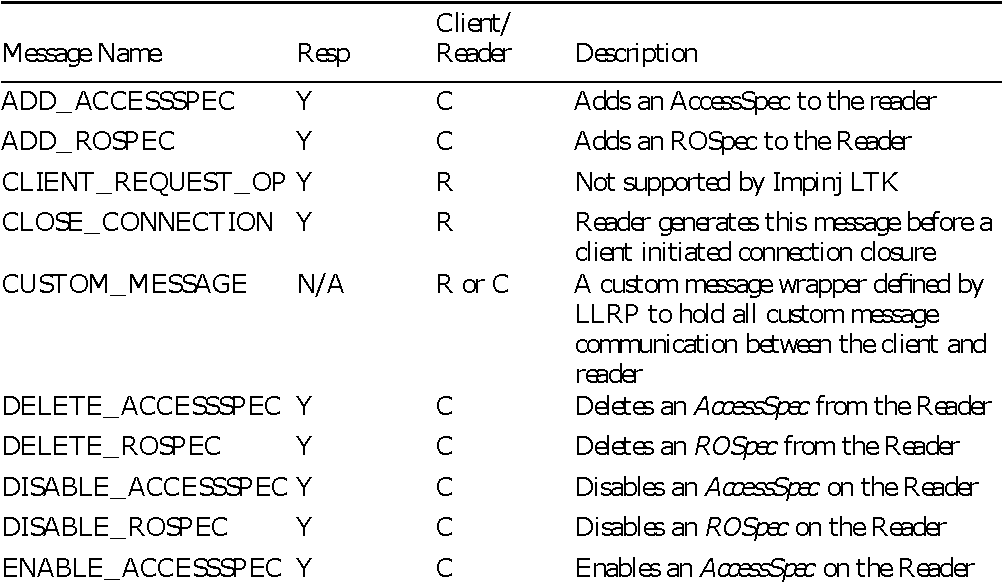
\includegraphics[width=\textwidth]{./figs/02-state-of-the-art/table_llrpmessages_1.pdf}
    \caption{\ac{llrp} Messages (except for responses)~\cite{ImpinjLTKProgrammers}} 
    \label{tab:llrpmessages1}
\end{table}


\begin{table}
    \centering
    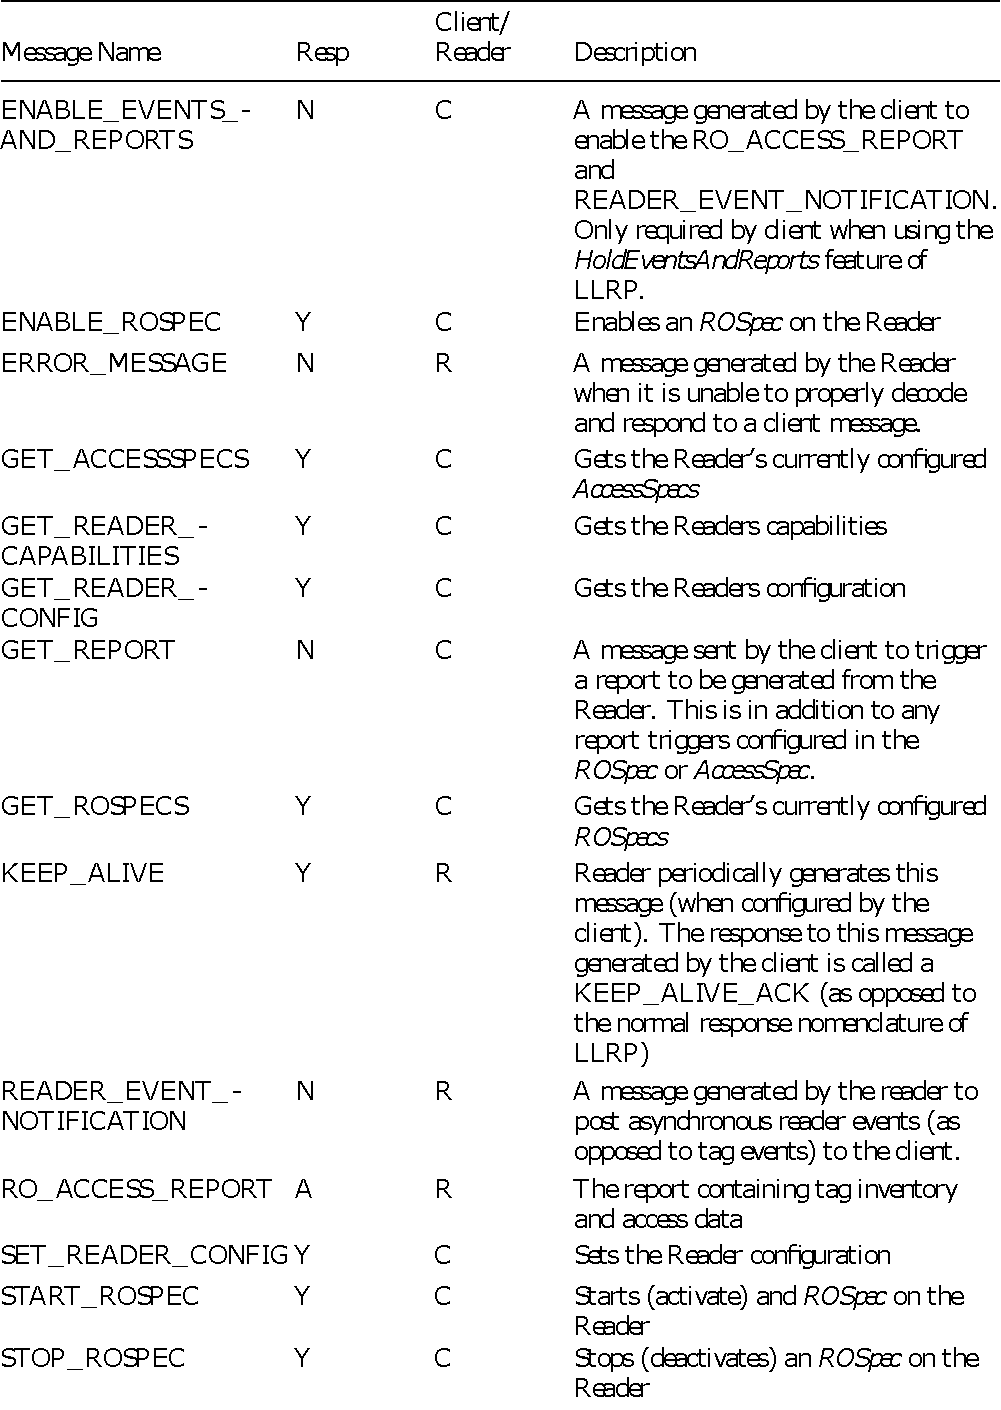
\includegraphics[width=\textwidth]{./figs/02-state-of-the-art/table_llrpmessages_2.pdf}
    \caption{\ac{llrp} Messages (except for responses)~\cite{ImpinjLTKProgrammers}} 
    \label{tab:llrpmessages2}
\end{table}

\end{appendices}